\section{Systemdenken \& Systemdynamik}
\subsection{Einführung}
\begin{multicols}{2}
	\subsubsection{Kausales Modell}
	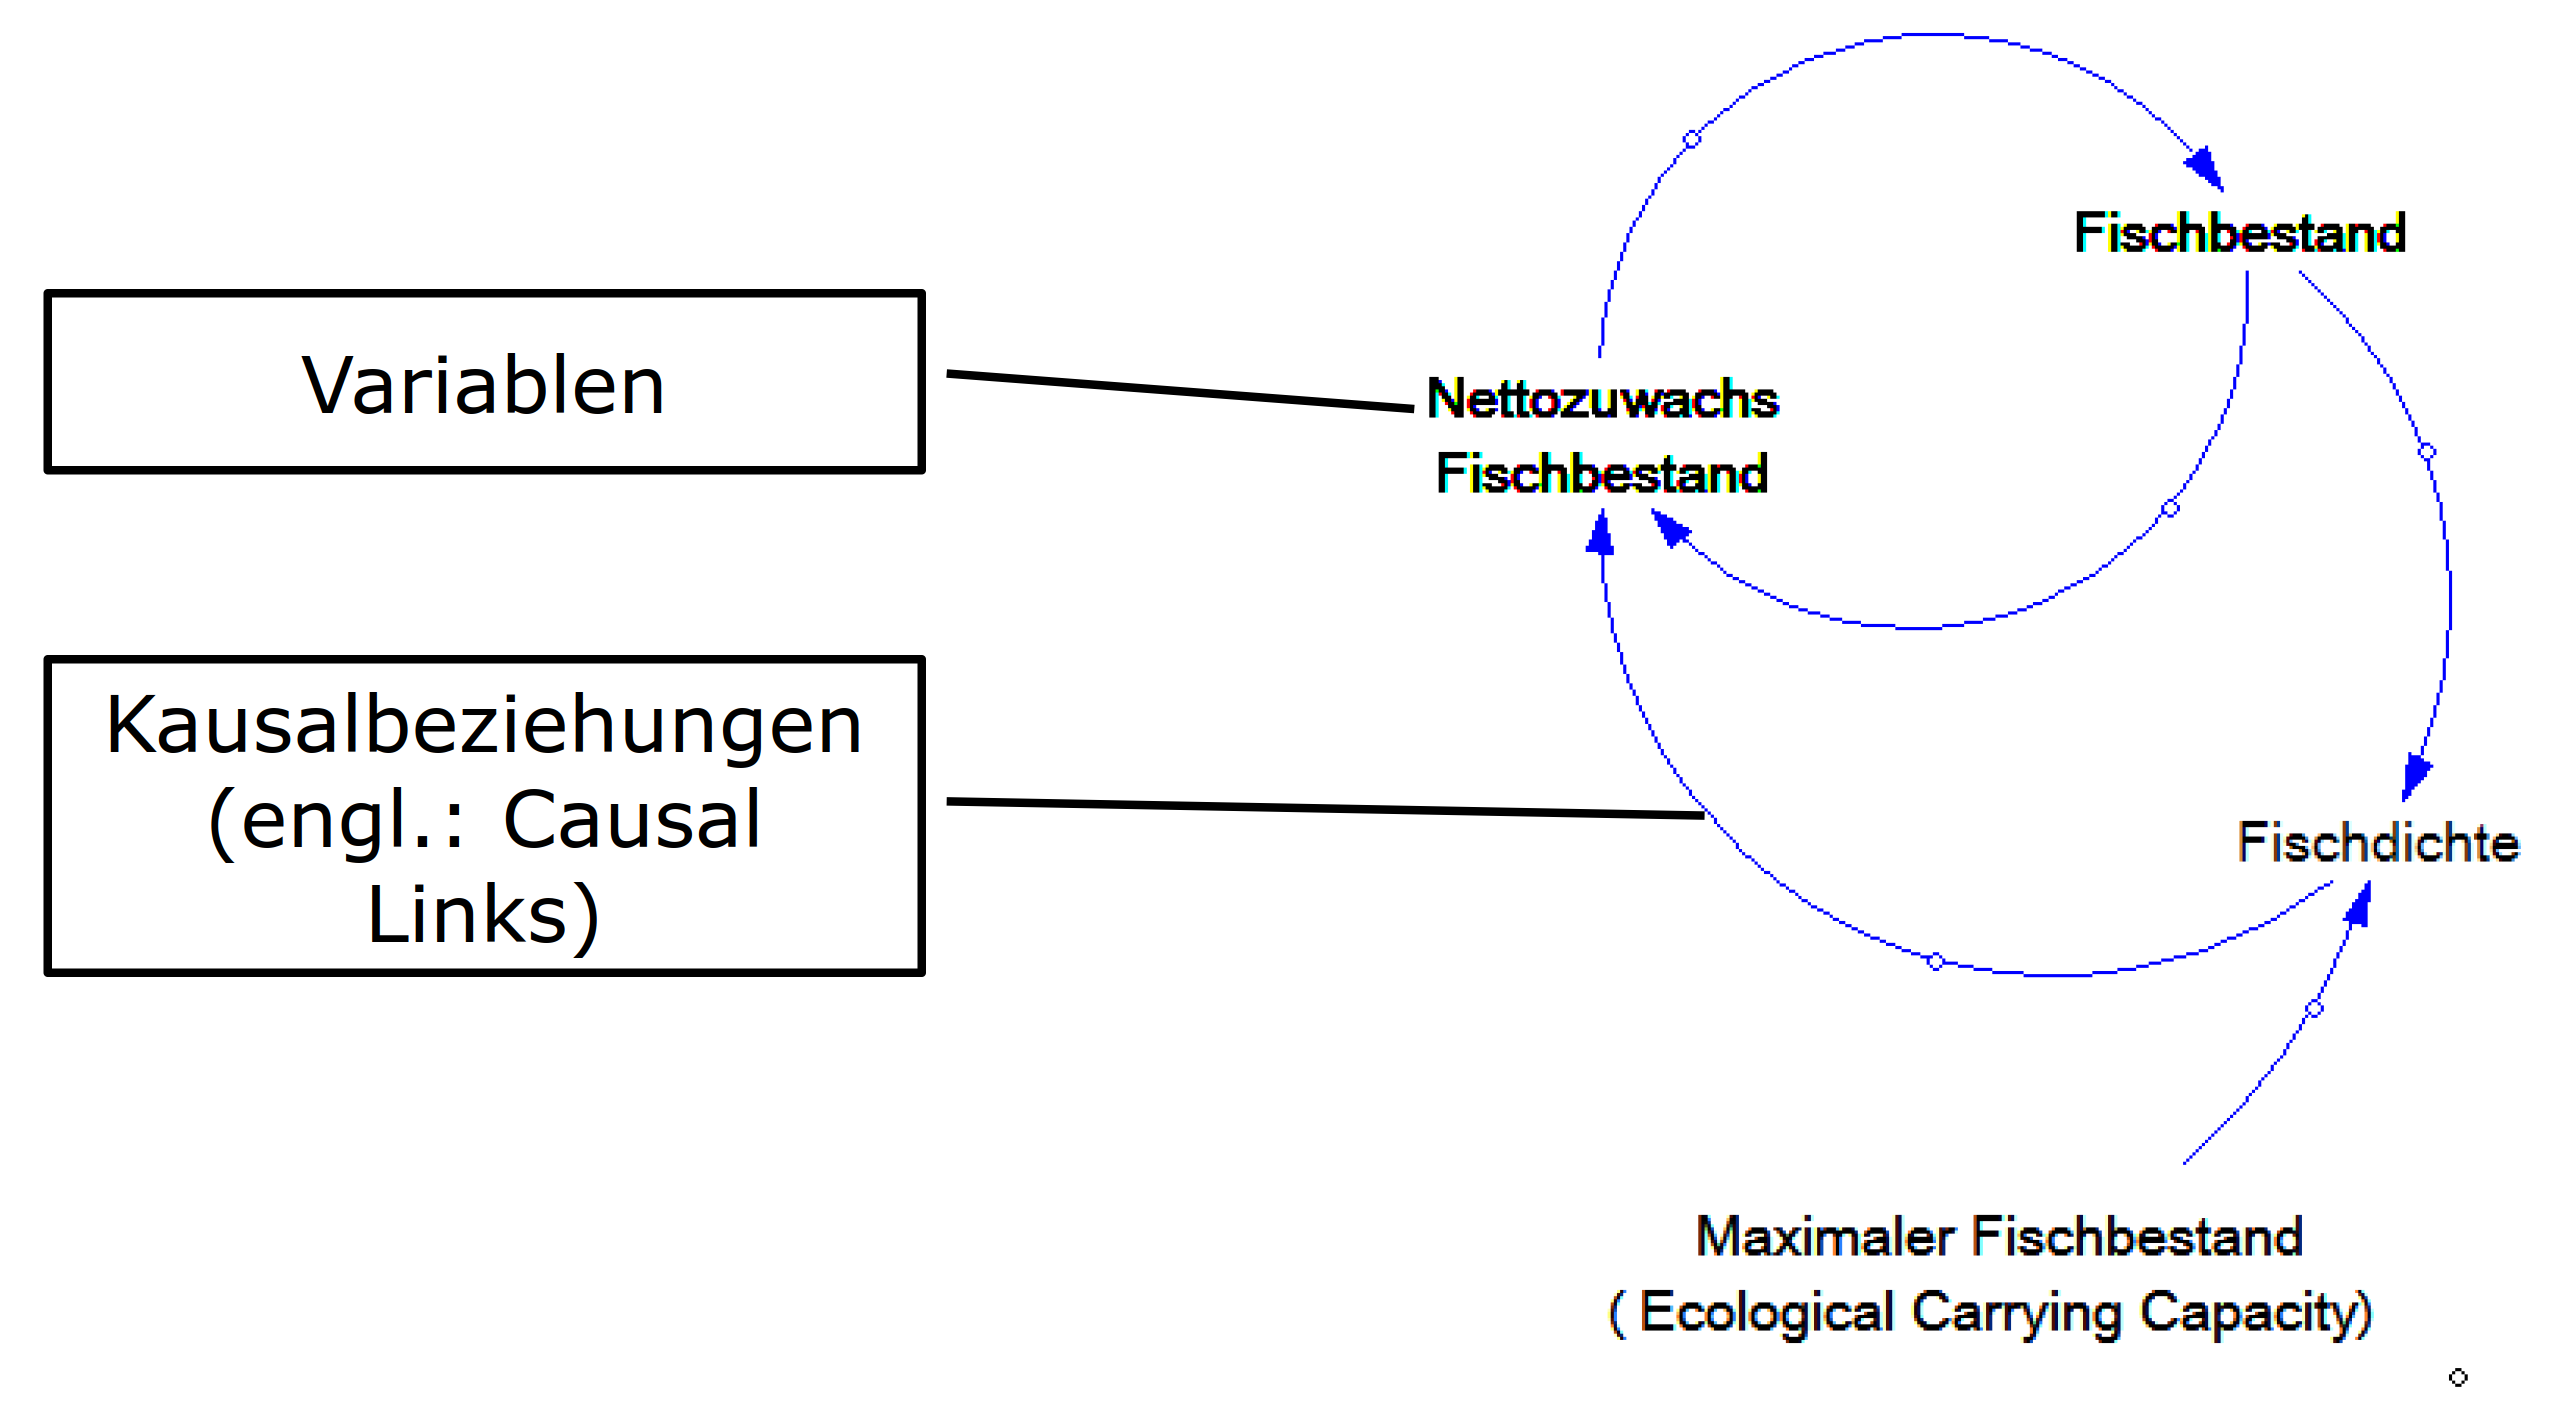
\includegraphics[width=0.5\textwidth]{pictures/kausales_modell}

	\subsubsection{Polarität einer Kausalbeziehung}
	\textbf{Positive Polarität:} Steigt (fällt) Ursache, dann steigt (fällt) Wirkung \\
	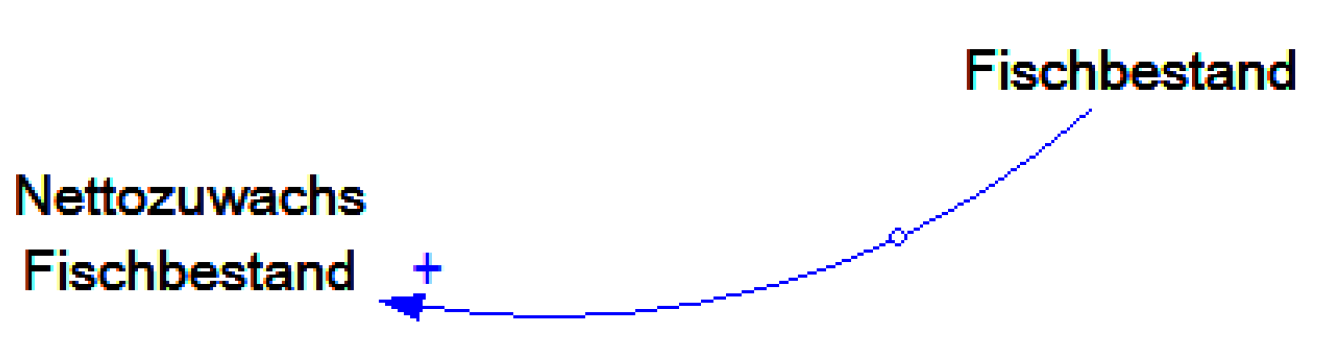
\includegraphics[width=0.35\textwidth]{pictures/positive_polaritaet}\\
	\textbf{Negative Polarität:} Steigt (fällt) Ursache, dann fällt (steigt) Wirkung \\
	
\includegraphics[width=0.35\textwidth]{pictures/negative_polaritaet}
\end{multicols}

\begin{multicols}{3}
	\subsubsection{Rückkopplung}
	Gerichteter Kreis von Kausalbeziehungen. \\
	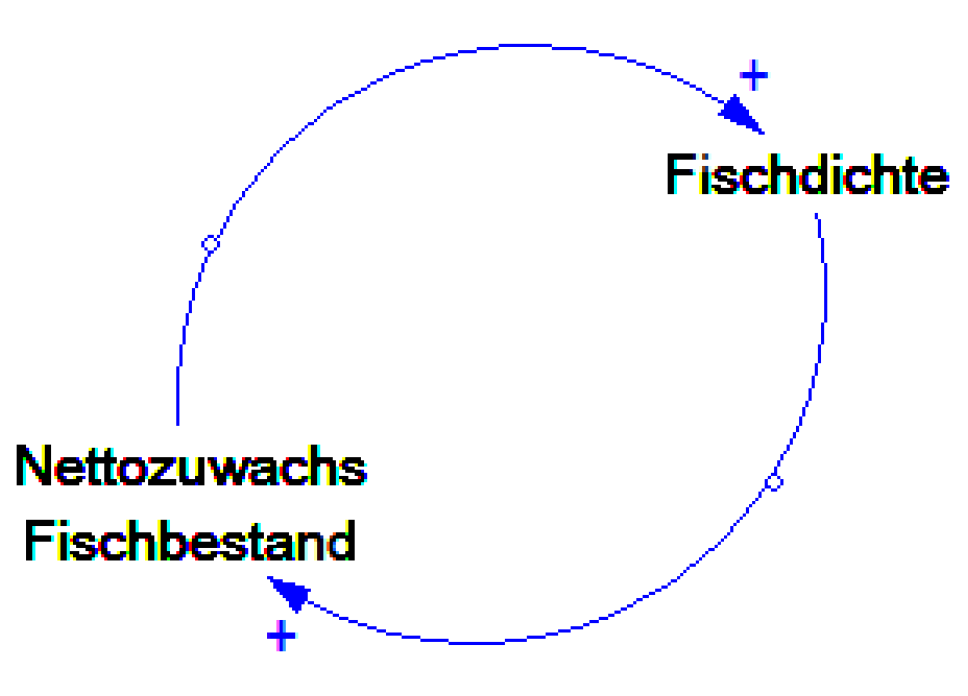
\includegraphics[width=0.25\textwidth]{pictures/rueckkopplung} \\
	
	\subsubsection{Selbstverstärkender Loop}
	Die Rückkoppelung verstärkt einen anfänglichen Effekt. \\
	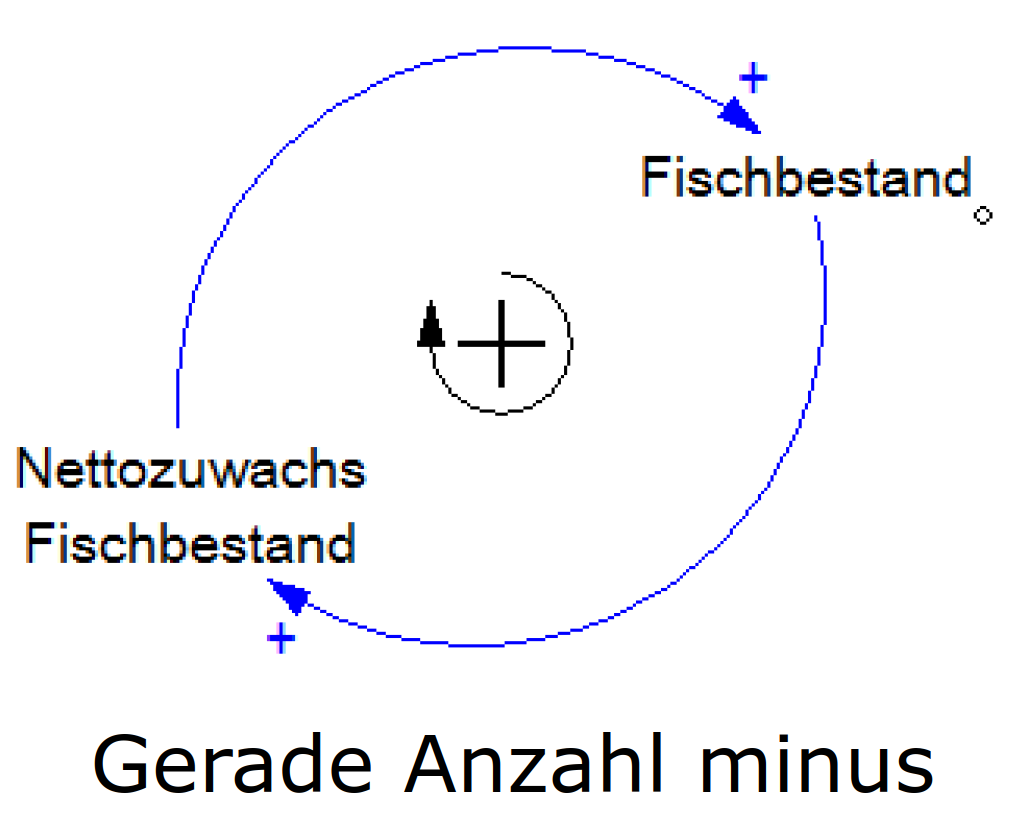
\includegraphics[width=0.25\textwidth]{pictures/selbstverstaerkender_loop}
	
	\subsubsection{Ausgleichender Loop}
	Die Rückkoppelung wirkt	einem anfänglichen Effekt entgegen.\\
	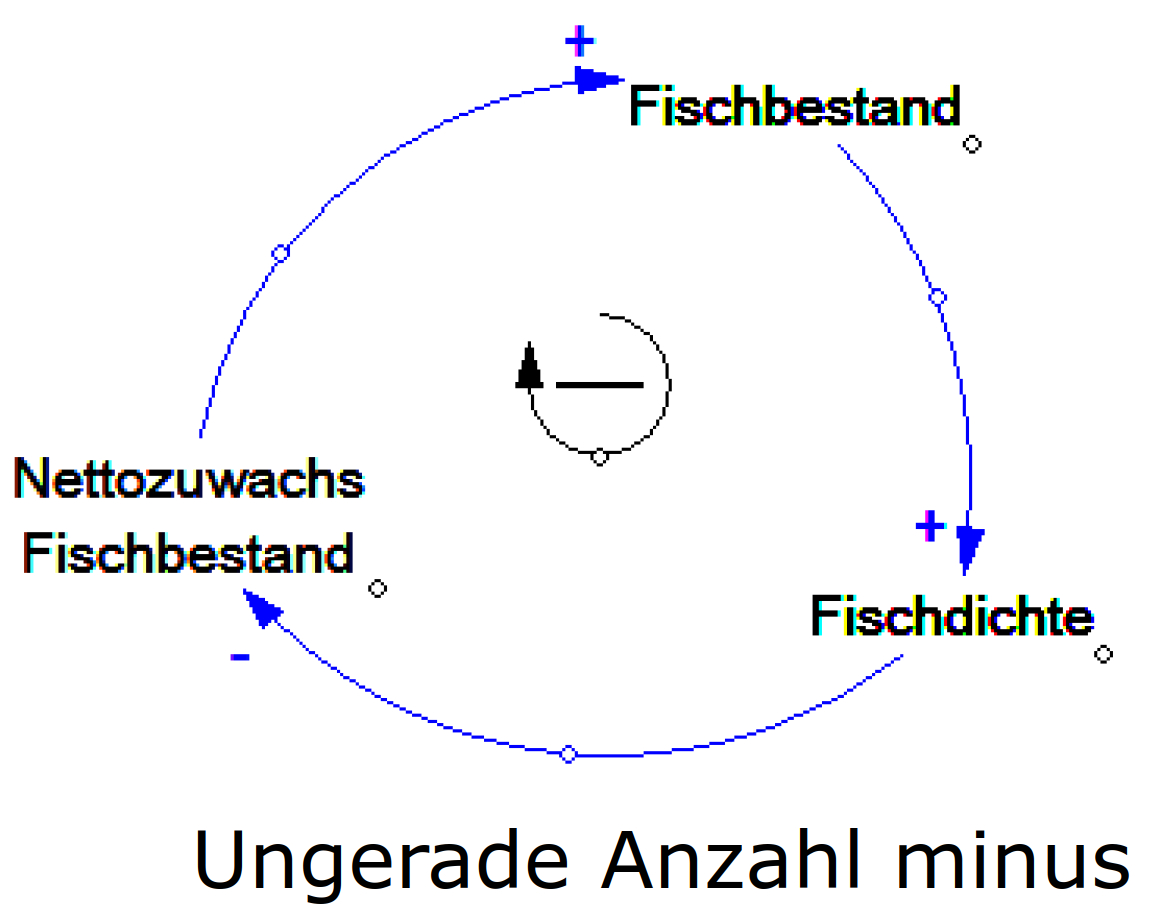
\includegraphics[width=0.25\textwidth]{pictures/ausgleichender_loop}
\end{multicols}	

\begin{multicols}{2}
	\subsubsection{Stock-and-Flow Diagramm}
	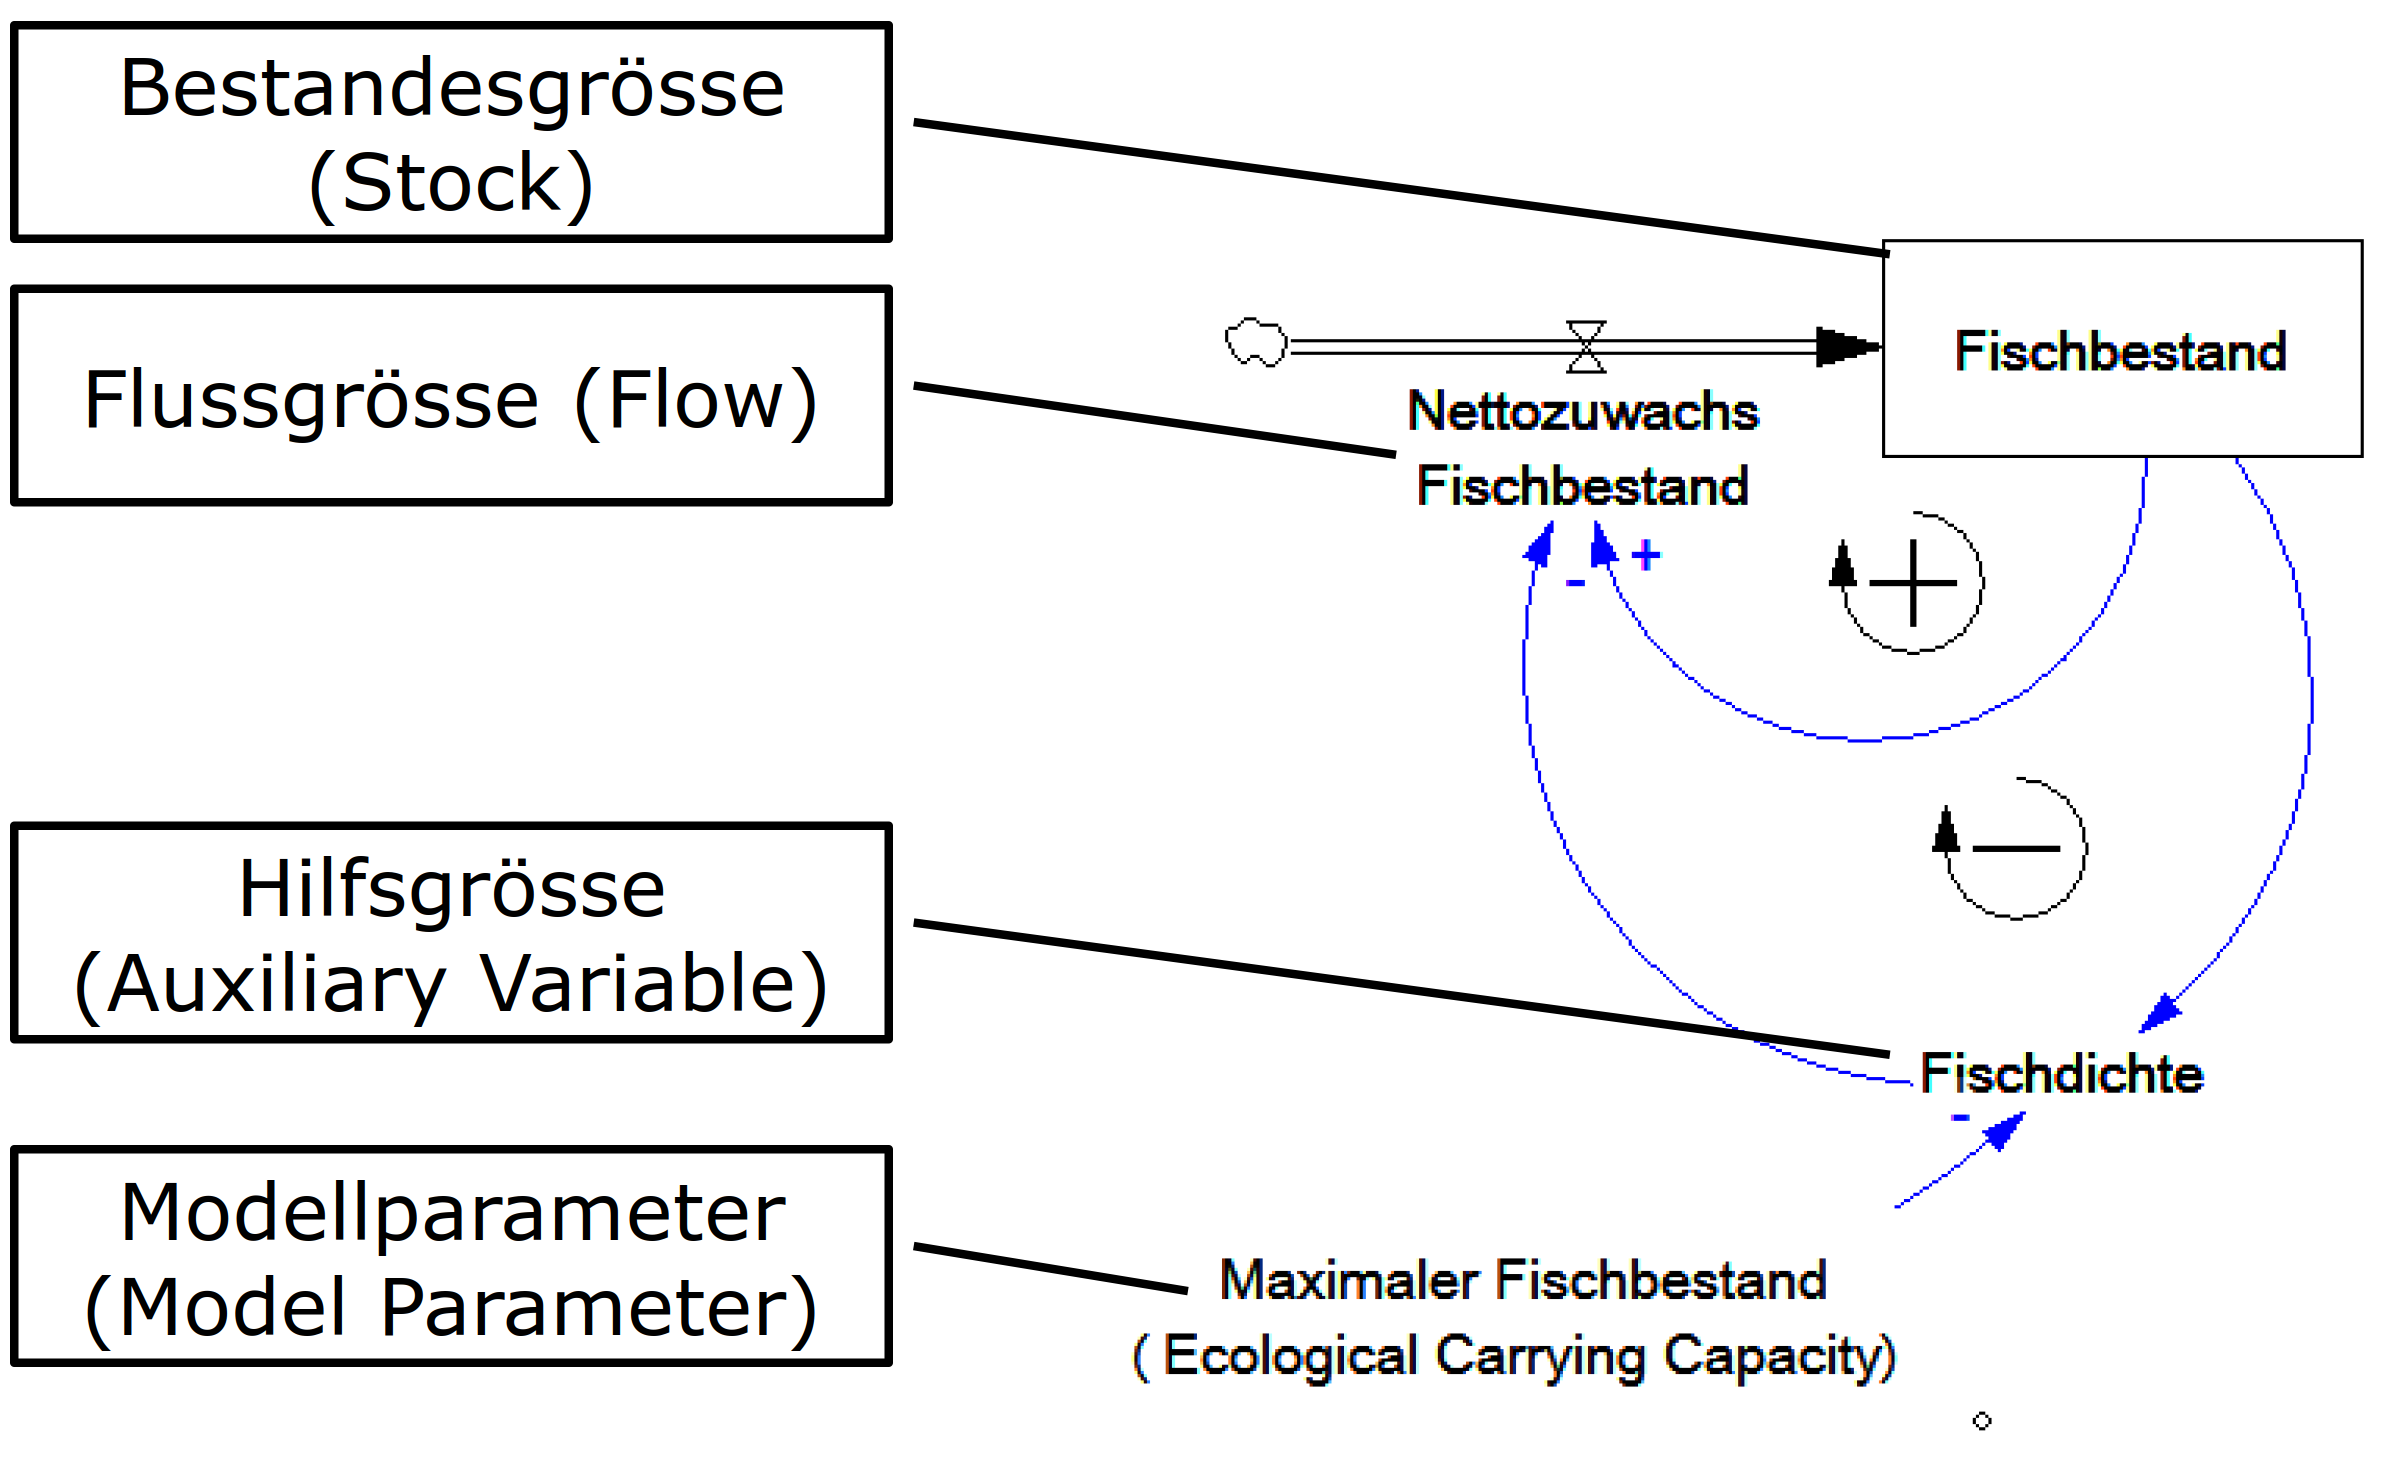
\includegraphics[width=0.5\textwidth]{pictures/stock_and_flow_diagramm}
	
	\subsubsection{Systemdynamisches Simulationsmodell}
	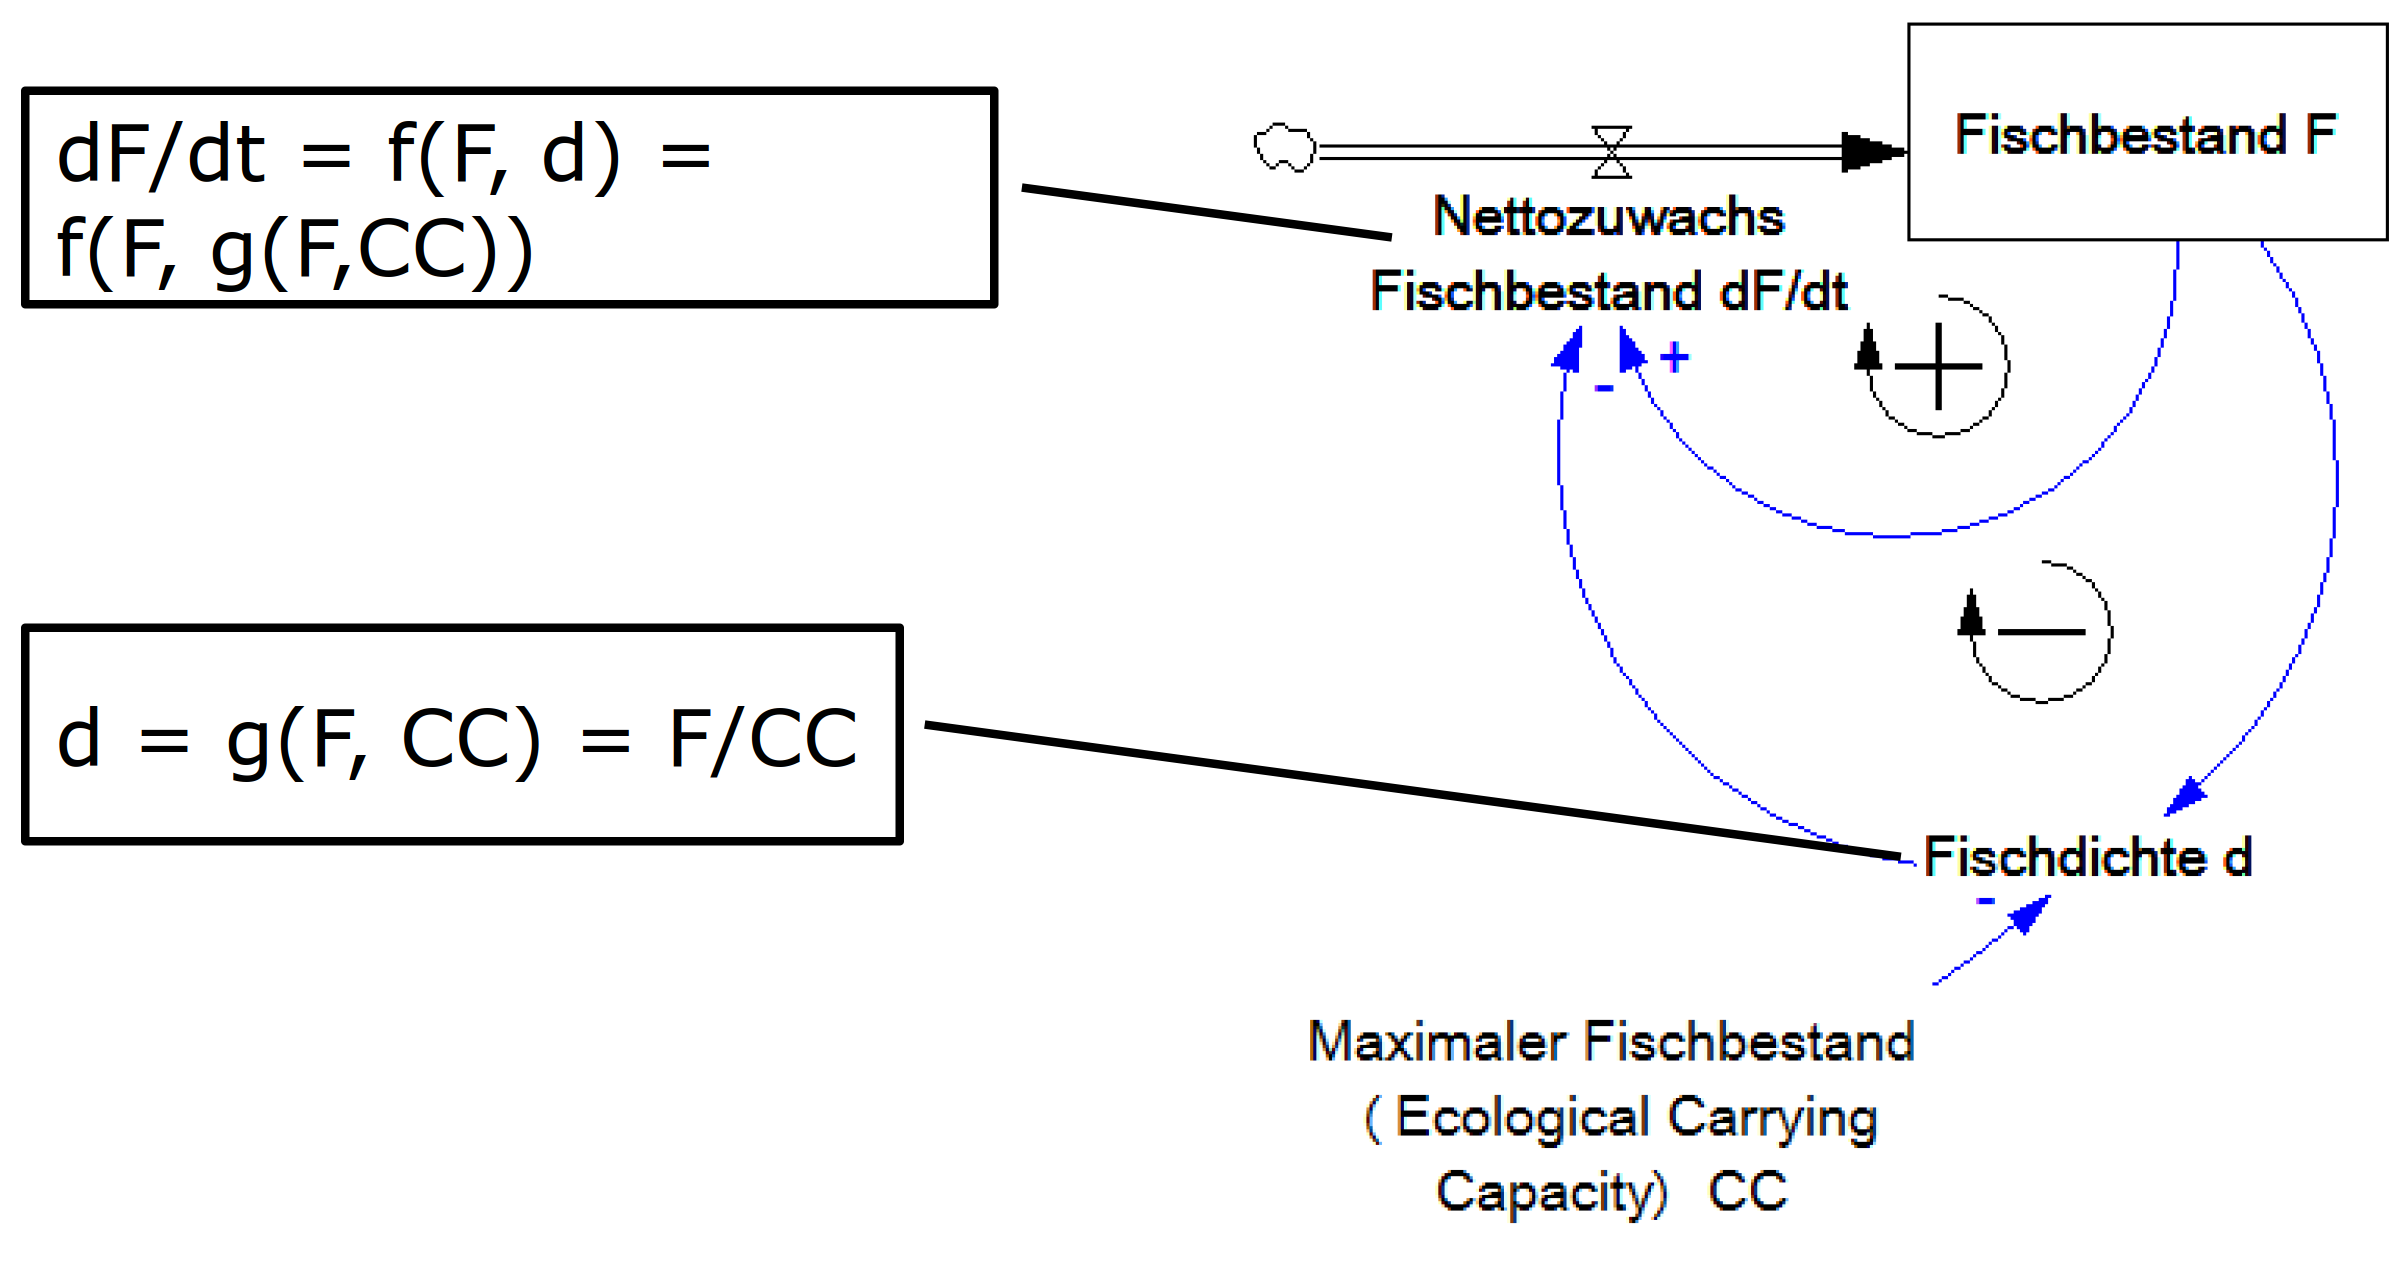
\includegraphics[width=0.5\textwidth]{pictures/systemdynamisches_simulationsmodell}
\end{multicols}	

\subsection{Grundideen}
\subsubsection{Ziele}
\begin{compactitem}
	\item \textbf{Verständnis, nicht Prognose} \\
	The goal of a system dynamics policy study is understanding – understanding the interactions in a complex system that are 	conspiring to create a problem, and understanding the structure	and dynamic implications of policy changes intended to improve	the system's behaviour (Richardson 1991: 164)
	\item \textbf{Modellieren, um zu lernen} \\
	Therefore, the primary goal is not to build the model of the system, but rather to get a group engaged in building a system dynamics model of a problem in order to see to what	extent this process might be helpful to increase problem understanding and to devise courses of action to which team members feel committed (Vennix 1996: 3).
\end{compactitem}

\subsubsection{Darstellungsformen}
\begin{compactenum}
	\item \textbf{Causal Loop Diagramme (\aszeichen{Kausaldiagramme})}
	\begin{compactitem}
		\item Kommunikations-Tool für ein gemeinsames mentales Modell und generelle Diskussionen
	\end{compactitem}
	\item \textbf{Stock-and-Flow Diagramme (\aszeichen{Flussdiagramme})}
	\begin{compactitem}
		\item Präzise Darstellung von Lagern (Stocks) und Raten (Flows)
	\end{compactitem}
	\item \textbf{Stock-and-Flow Diagramme mit Formeln}
	\begin{compactitem}
		\item Formulierung sämtlicher Flüsse als Formeln
		\item Erlaubt quantitative Simulation
	\end{compactitem}
\end{compactenum}

\subsubsection{Computersimulation}
\begin{compactitem}
	\item Die Dynamik von Feedbackmodellen korrekt interpretieren
	\item Nicht antizipierte Nebenwirkungen entdecken
	\item Modellanalyse
	\begin{compactitem}
		\item Sensitivitätsanalyse von Parametern und funktionalen Beziehungen
		\item Einfluss unterschiedlicher Modellformulierungen
		\item Massnahmenanalyse (Policy Analysis)
	\end{compactitem}
\end{compactitem}

\subsection{Akkumulation}